\documentclass{article}

\usepackage{amsmath,amssymb}
\usepackage{tikz}
\usepackage{pgfplots}
\usepackage{xcolor}
\usepackage[left=2.1cm,right=3.1cm,bottom=3cm,footskip=0.75cm,headsep=0.5cm]{geometry}
\usepackage{enumerate}
\usepackage{enumitem}
\usepackage{marvosym}
\usepackage{tabularx}
\usepackage[amsmath,thmmarks,standard]{ntheorem}
\usepackage{mathtools}

\usepackage[utf8]{inputenc}

\renewcommand*{\arraystretch}{1.4}
\newcommand{\E}{\mathbb{E}}

\newcolumntype{L}[1]{>{\raggedright\arraybackslash}p{#1}}
\newcolumntype{R}[1]{>{\raggedleft\arraybackslash}p{#1}}
\newcolumntype{C}[1]{>{\centering\let\newline\\\arraybackslash\hspace{0pt}}m{#1}}

\DeclareMathOperator{\tr}{tr}
\DeclareMathOperator{\Var}{Var}
\DeclareMathOperator{\Cov}{Cov}
\renewcommand{\E}{\mathbb{E}}

\newtheorem{thm}{Theorem}
\newtheorem{lem}{Lemma}

\title{\textbf{Einführung in die Produktion, Tutorium 2}}
\author{\textsc{Henry Haustein}}
\date{}

\begin{document}
	\maketitle
	
	\section*{Aufgabe 3}
	\begin{enumerate}[label=(\alph*)]
		\item Zielfunktion: $1\cdot r_1 + 1\cdot r_2 \to \min$ unter der Nebenbedingung $11=12r_1 - 4r_1^2 + 4r_1r_2 - 4r_2^2$. Der Lagrangeansatz ist damit $L = r_1+r_2+\lambda (12r_1-4r_1^2 + 4r_1r_2 - 4r_2^2 - 11)$.
		\begin{align}
			\frac{\partial L}{\partial r_1} &= 1 + 12\lambda - 8\lambda r_1 + 4\lambda r_2 = 0 \\
			\frac{\partial L}{\partial r_2} &= 1 + 4\lambda r_1 - 8\lambda r_2 = 0 \\
			\frac{\partial L}{\partial r_1} &= 12r_1-4r_1^2 + 4r_1r_2 - 4r_2^2 - 11 = 0
		\end{align}
		Gleichsetzen von (1) und (2) ergibt
		\begin{align}
			 + 12\lambda - 8\lambda r_1 + 4\lambda r_2 &= 1 + 4\lambda r_1 - 8\lambda r_2 \notag \\
			 12 - 8r_1 + 4r_2 &= 4r_1 - 8r_2 \notag \\
			 12 + 12r_2 &= 12r_1 \notag \\
			 1 + r_2 &= r_1 \notag
		\end{align}
		\item Dazu leiten wir die Produktionsfunktion $x$ nach $r_1$ und $r_2$ ab und setzen sie 0:
		\begin{align}
			\frac{\partial x}{\partial r_2} = -8r_2 + 4r_1 &= 0 \notag \\
			4r_1 &= 8r_2 \notag \\
			r_1 &= 2 r_2 \notag
		\end{align}
		bzw.
		\begin{align}
			\frac{\partial x}{\partial r_1} = 4r_2 - \underbrace{8r_1}_{16r_2} + 12 &= 0 \notag \\
			-12 r_2 + 12 &= 0 \notag \\
			r_2 &= 1 \notag \\
			\Rightarrow r_1 &= 2 \notag
		\end{align}
		\item Für die Minimalkostenkombination nutzen wir unsere Erkenntnisse aus (a) und setzen dies in (3) ein:
		\begin{align}
			\underbrace{12r_1}_{12+12r_2}-4\underbrace{r_1^2}_{1+2r_2+r_2^2} + 4\underbrace{r_1}_{1+r_2}r_2 - 4r_2^2 - 11 &= 0 \notag \\
			12 + 12r_2 - 4 - 8r_2 - 4r_2^2 + 4r_2 + 4r_2^2 - 4r_2^2 - 11 &= 0 \notag \\
			-4r_2^2 + 8r_2 - 3 &=0 \notag \\
			r_{2a} &= 0.5 \notag \\
			r_{2b} &= 1.5 \notag
		\end{align}
		$r_{2b}$ ist Faktorverschwendung, also ist $r_2=0.5$ und entsprechend $r_1=1.5$. Die Kosten betragen dann 2 und der Lagrange-Multiplkator $\lambda$ hat dann den Wert (mit Gleichung (2) berechnet)
		\begin{align}
			1 + 4\lambda\cdot 1.5 - 8\lambda\cdot 0.5 &= 0 \notag \\
			\lambda &= 0.5 \notag
		\end{align}
	\end{enumerate}

	\section*{Aufgabe 4}
	\begin{enumerate}[label=(\alph*)]
		\item Die Isoquante ist
		\begin{center}
			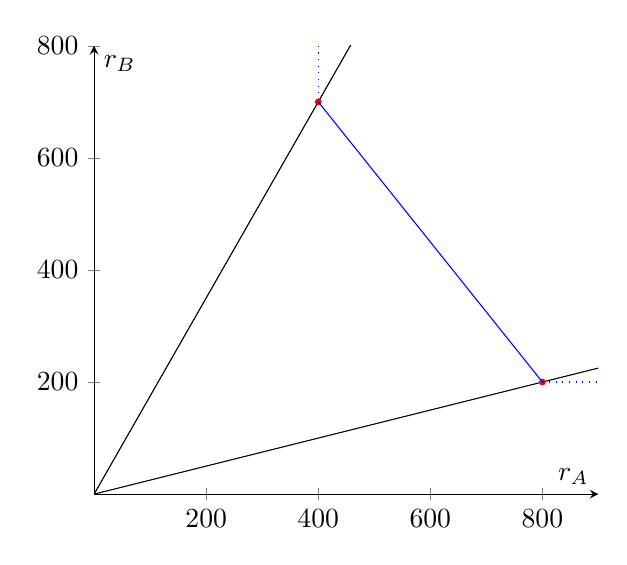
\begin{tikzpicture}
				\begin{axis}[
					xmin=0, xmax=900, xlabel=$r_A$,
					ymin=0, ymax=800, ylabel=$r_B$,
					samples=400,
					axis x line=middle,
					axis y line=middle,
					domain=0:900,
					axis equal image
					]
					\addplot[mark=none,smooth,black] {1.75*x};
					\addplot[mark=none,smooth,black] {0.25*x};
					
					\draw[red,fill=red,radius=5] (axis cs: 400,700) circle;
					\draw[red,fill=red,radius=5] (axis cs: 800,200) circle;
					
					\draw[blue,dotted] (axis cs: 400,800) -- (axis cs: 400,700);
					\draw[blue] (axis cs: 400,700) -- (800,200);
					\draw[blue,dotted] (axis cs: 800,200) -- (900,200);
					
				\end{axis}
			\end{tikzpicture} \\
			\textcolor{blue}{Isoquante für $x=200$}
		\end{center}
		\item Mit der 2-Punkte-Gleichung ergibt sich
		\begin{align}
			y-y_1 &= \frac{y_2-y_1}{x_2-x_1} \cdot (x-x_1) \notag \\
			y &= \frac{200-700}{800-400}(x-400) + 700 \notag \\
			&= -1.25x + 400 + 700 \notag \\
			&= -1.25x + 1200 \quad (400\le x\le 800) \notag
		\end{align}
		\item Die Kostenfunktion ist $K=2r_A + 2.5r_B$. Eine Gleichung für $r_B$ haben wir schon in (b) ermittelt. Einsetzen liefert:
		\begin{align}
			K &= 2r_A + 2.5(-1.25r_A + 1200) \notag \\
			&= 2r_A - 3.125r_A + 3000 \notag \\
			&= -1.125r_A + 3000 \notag
		\end{align}
		Da $K$ minimiert werden soll, muss $r_A$ maximiert werden, also wählen wir $r_A=800$. Damit folgt dann $r_B=200$ und $K=2100$.
		\begin{center}
			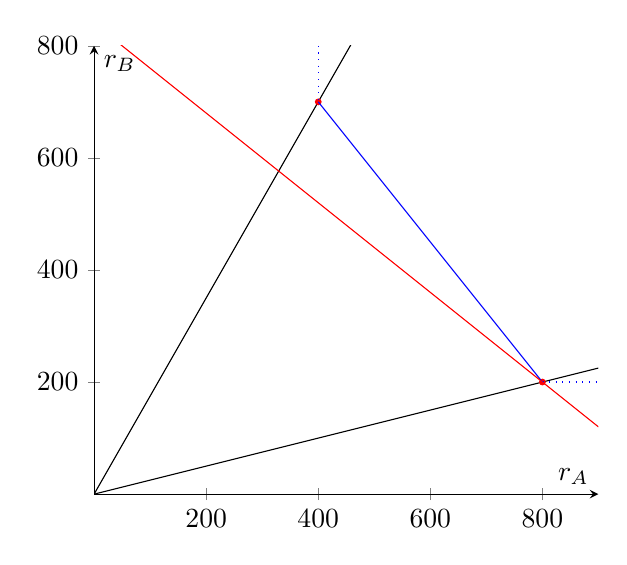
\begin{tikzpicture}
				\begin{axis}[
					xmin=0, xmax=900, xlabel=$r_A$,
					ymin=0, ymax=800, ylabel=$r_B$,
					samples=400,
					axis x line=middle,
					axis y line=middle,
					domain=0:900,
					axis equal image
					]
					\addplot[mark=none,smooth,black] {1.75*x};
					\addplot[mark=none,smooth,black] {0.25*x};
					
					\draw[red,fill=red,radius=5] (axis cs: 400,700) circle;
					\draw[red,fill=red,radius=5] (axis cs: 800,200) circle;
					
					\draw[blue,dotted] (axis cs: 400,800) -- (axis cs: 400,700);
					\draw[blue] (axis cs: 400,700) -- (800,200);
					\draw[blue,dotted] (axis cs: 800,200) -- (900,200);
					
					\addplot[mark=none,smooth,red] {-0.8*x + 840};
					
				\end{axis}
			\end{tikzpicture} \\
			\textcolor{blue}{Isoquante für $x=200$}, \textcolor{red}{Kostenfunktion}
		\end{center}
	\end{enumerate}
	
\end{document}